\documentclass[a4paper,10pt]{article}
\usepackage[utf8]{inputenc}


\usepackage[UKenglish]{babel}
\usepackage[utf8]{inputenc}
\usepackage{amsmath}
\usepackage{csquotes}
\usepackage{amssymb}
\usepackage{color}

\usepackage{mathtools}
\DeclarePairedDelimiter{\ceil}{\lceil}{\rceil}
\DeclarePairedDelimiter{\floor}{\lfloor}{\rfloor}

% date format
\usepackage[ddmmyyyy]{datetime}
\renewcommand{\dateseparator}{/}

\usepackage{listings}
\lstdefinestyle{mono}{
  basicstyle=\small\ttfamily,
  columns=flexible,
  breaklines=true
}

\usepackage{tabularx}
\newcommand{\specialcell}[2][c]{%
  \footnotesize{\begin{tabular}[#1]{@{}c@{}}#2\end{tabular}}}

\newcommand{\red}[1]{\textcolor{red}{#1}}
\newcommand{\blue}[1]{\textcolor{blue}{#1}}

\usepackage[inline]{enumitem}

%opening
\title{\vspace*{\fill}COMP90007 Internet Technologies\\Final Semester Summary\vspace*{\fill}}
\author{Frederick Zhang}

\begin{document}

\begin{titlepage}
  \maketitle
  \thispagestyle{empty}
\end{titlepage}

\section*{Chapter 1. Introduction}
\begin{enumerate}
  \item What are the Internet and the WWW?
    \newline The Internet is a network of networks.
    \newline The WWW is a distributed system that runs on the top of the Internet.
  
  \item Type of Networks (Section 1.2)
    \begin{enumerate}
      \item Personal Area Networks
      \item Local Area Networks
      \item Metropolitan Area Networks
      \item Wide Area Networks
      \item Internetworks
    \end{enumerate}
  
  \item Network Hierarchies (Section 1.3.1)
    \newline To reduce their design complexity, most networks are organized as a stack of \red{layers} or \red{levels}, each one built upon the one below it. The purpose of each layer is to offer certain \red{services} to higher layers while shielding those layers from details of how the offered services are actually implemented.
  
  \item Layers, Protocols and Interfaces (Section 1.4)
    \newline Seven layers of OSI (up to bottom): Application, Presentation, Session, Transport, Network, Data Link, Physical
    \newline Four layers of TCP/IP (up to bottom): Application, Transport, Internet, Link
    \newline Five layers used in book: Application, Transport, Network, Link, Physical
    \newline
    \newline A \red{protocol} is an agreement between the communicating parties on how communication is to proceed.
    \newline Between each pair of adjacent layers is an \red{interface}. The interface defines which primitive operations and services the lower layer makes available to the upper one. 
  
  \item Connection-oriented and Connectionless
    \newline Connection-oriented service is modelled after the telephone system. To use a connection-oriented network service, the service user first \red{establishes} a connection, uses the connection, and then \red{releases} the connection. In some cases when a connection is established, the sender, receiver and subnet conduct a \red{negotiation} about the parameters to be used.
    \newline Connectionless service is modelled after the postal system. Each \red{packet} carries the full destination address, and each one is routed through the intermediate nodes inside the system independent of all subsequent messages. When the intermediate nodes receive a message in full before sending it on to the next node, this is called \red{store-and-forward switching}. The alternative, in which the onward transmission of a message at a node starts before it is completely received by the node, is called \red{cut-through switching}.
  
  \item Service Primitives (1.3.3, 1.3.4, 1.3.5)
    \newline\textit{Connection-oriented and Connectionless}: check previous section.
    \newline
    \newline A \red{service} is formally specified by a set of \red{primitives} (operations) available to user processes to access the service. If the \red{protocol stack} is located in the operating system, the \red{primitives} are normally system calls.
    \newline
    \newline Primitives in \red{Berkeley socket} interface: \texttt{LISTEN}, \texttt{CONNECT}, \texttt{ACCEPT}, \texttt{RECEIVE}, \texttt{SEND}, \texttt{DISCONNECT}.
    \newline
    \newline\textit{DIFFERENCES BETWEEN SERVICE AND PROTOCOL}
    \begin{itemize}
      \item A \red{service} is a set of \red{primitives} (operations) that a layer provides to the layer above it. A \red{protocol}, in contrast, is a set of rules governing the format and meaning of packets, or messages that are exchanged by the peer entities within a layer.
      \item A \red{service} is like an abstract data type or an object but does not specify how these operations are implemented. In contrast, a \red{protocol} relates to the implementation of the service and as such is not visible to the user of the service.
    \end{itemize}
  
  \item Network Reference Models (TCP/IP and OSI Reference) (1.4.1, 1.4.2 and 1.4.3)
    \begin{enumerate}
      \item\textit{DIFFERENCES BETWEEN OSI AND TCP/IP}
        \begin{itemize}
          \item The biggest contribution of the OSI model is that it makes the \red{distinction} between the three concepts of Services, Interfaces and Protocols explicit.
            \newline Each layer performs some services for the layer above it.
            \newline A layer's interface tells the processes above it how to access it.
            \newline The peer protocols used in a layer are the layer's own business.
          \item The TCP/IP model did not originally clearly distinguish between Services, Interfaces and Protocols (although people have tried to retrofit it after the fact to make it more OSI-like).
          \item CO \& CL Support in OSI and TCP/IP
            \newline\begin{tabular}{l | l | l}
              & Network Layer & Transport Layer \\ \hline
              OSI & CO \& CL & CO \\
              TCP/IP & CL & CO \& CL
            \end{tabular}
        \end{itemize}
      \item Disadvantages of OSI (Why OSI did not take over the world)
        \begin{itemize}
          \item Bad timing
            \begin{itemize}
              \item TCP/IP adopted before OSI was even formalized. Vendors did not want to support 2nd standard.
              \item 2-elephant graph: The research period of OSI was too long and it was not standardized when large investments came. However, the academic market was large enough that many vendors had begun cautiously offering TCP/IP products
            \end{itemize}
          \item Bad technology
            \begin{itemize}
              \item Being incomprehensible: two of the layers (session and presentation) are nearly empty, whereas two other ones (data link and network) are overfull.
              \item Some functions, such as addressing, flow control, and error control, reappear again and again in each layer.
            \end{itemize}
          \item Bad implementation
            \begin{itemize}
              \item The initial implementations were inefficient compared with TCP/IP.
              \item Less community support.
            \end{itemize}
          \item Bad politics
            \begin{itemize}
              \item OSI was widely perceived as the product of quasi-government standards processes rather than driven by good design processes
            \end{itemize}
        \end{itemize}
      \item Disadvantages of TCP/IP
        \begin{itemize}
          \item The model does not clearly distinguish the concepts of services, interfaces, and protocols.
          \item The model is not at all general and is poorly suited to describing any protocol stack other than TCP/IP.
          \item The link layer is not really a layer but an interface (between the network and data link layers).
          \item The model does not distinguish between physical and data link layers.
          \item Early implementations were fragile.
        \end{itemize}
      \item Example Question
        \newline Briefly explain the design principles and benefits of the Open System Interconnection (OSI) Layer Division approach (and layered approaches in general) for network design.
        \begin{enumerate}
          \item Principles
          \begin{itemize}
            \item A layer should be created where a different abstraction is needed
            \item Each layer should perform a well defined function
            \item The function of each layer should be chosen with a view toward defining internationally standardized protocols
            \item The layer boundaries should be chosen to minimize the information flow access the interfaces.
            \item The number of layers should be large enough that distinct functions need not to be thrown together in the same layer out of necessity, and small enough that the architecture does not become unwieldy.
          \end{itemize}
          \item Benefits
            \begin{itemize}
              \item Break up the design problem into smaller
              \item Protocols can be changed without affecting higher or lower ones
            \end{itemize}
          \item Disadvantage
            \begin{itemize}
              \item Information at one layer may not be available to other layers, e.g., the timestamp on a packet.
              \item Duplication of functions can occur between layers, e.g., buffering or error control.
              \item Optimization of functions is difficult between layers, e.g., providing error detection at the link or transport layers.
            \end{itemize}
        \end{enumerate}
      \end{enumerate}
\end{enumerate}
    
\newpage\section*{Chapter 2. The Physical Layer}
\begin{enumerate}
  \item Nyquist Theorem \& Shannon's Theorem(2.1.3)
    \begin{itemize}
      \item $ maximum\ data\ rate = 2B\log_2 V\ (bits/sec) $
      \item $ maximum\ data\ rate = B\log_2 (1+S/N)\ (bits/sec) $
    \end{itemize}
    We call the rate at which the signal changes the \red{symbol rate} to distinguish it from the \red{bit rate}. The bit rate is the symbol rate multiplied by the number of bits per symbol. An older name for the symbol rate is the \red{baud rate}.
  
  \item Latency \& Delay
    \newline Latency is the time delay associated with sending a message over a link.
    \newline This is make of up two parts
    \begin{itemize}
      \item Transmission Delay
        \newline $ \textit{T-delay} = Message\ in\ bits/Rate\ of\ transmission \\= M/R\ seconds $
      \item Propagation Delay
        \newline $ \textit{P-delay} = Length\ of\ the\ channel/Speed\ of\ signals \\= Length/Speed\ of\ signal $
      \item $ Lentency = L = M/R + \textit{P-delay} $
    \end{itemize}
    
  \item Guided Media - Copper vs Fiber (2.2.3, 2.2.4)
    \begin{itemize}
      \item [Copper] Cheaper, no specialist skills required
      \item [Fiber] Higher bandwidths, greater distance between repeaters (5km vs 50km), not physically influenced by interferences or surges, thin/lightweight, no leakage, difficult to tap
    \end{itemize}
\end{enumerate}

\newpage\section*{Chapter 3. The Data Link Layer}
\begin{enumerate}
  \item Design Issues (3.1)
    \newline Units, Services, Framing
    \newline
    \newline\textit{FUNCTIONS OF DATA LINK LAYER}
    \begin{itemize}
      \item Providing a well-defined service interface to the network layer
      \item Dealing with transmission errors
      \item Regulating the flow of data so that slow receivers are now swamped by faster senders
    \end{itemize}
  
  \item Framing (3.1.2)
    \newline To make it easy for a receiver to find the start of new frames while using little of the channel bandwidth:
    \begin{itemize}
      \item Byte/Character count
      \item Flag bytes with byte stuffing
      \item Flag bits with bit stuffing
      \item Physical layer coding violations
    \end{itemize}
  
  \item Flow Control and Error Control (3.1.3, 3.1.4)
    \begin{enumerate}
      \item Flow control
      \begin{itemize}
        \item Feedback control
        \item Rate based
      \end{itemize}
      \item Error correcting
      \begin{itemize}
        \item Hamming code
        \item Binary convolutional codes
        \item Reed-Solomon codes
        \item Low-Density Parity Check code
      \end{itemize}
      \item Hamming code
      \begin{itemize}
        \item $ n = m + r $ ($ codeword = message + check $)
        \item $ d + 1 $ (detecting), $ 2d + 1 $ (correcting)
        \item correct one $\rightarrow$ $ (n + 1)2^m \leq 2^n $ $\rightarrow$ $ (m + r +1) \leq 2^r $
      \end{itemize}
      \item Error detecting
      \begin{itemize}
        \item Parity
        \item Checksum, e.g., 16-bit internet in IP, Flectcher's checksum
        \item CRC
      \end{itemize}
    \end{enumerate}

  \newpage\item Flow Control Protocols
    \newline\begin{table}[h]\begin{tabularx}{\textwidth}{l | r | X | X}
      & Utilization & Pros & Cons \\ \hline
      Stop and Wait & 50\% & & \\ \hline
      One Bit & 100\% & & Synchronization issues \\ \hline
      Go-Back-N & 100\% & Senders do not need to wait for ACK before sending next & Receiver discard all subsequent frames from error point, sending no ACK, until the next frame in sequence \\ \hline
      Selective Repeat & 100\% & Cumulative ACK\newline NAK & Receiver needs more buffer
    \end{tabularx}\end{table}
    
  \item Link Utilization Formula
    \newline\texttt{B}: bit-rate of the link (bit/sec)
    \newline\texttt{L}: length of the frame (bit)
    \newline $ T_f = Time\ needed\ to\ transmit\ a\ frame\ of\ length\ L $
    \newline $ T_p = Propagation\ delay\ of\ the\ channel $ (unit: sec)
    \newline $ T_a = Time\ for\ transmitting\ an\ ACK $ (assume this is zero)
    \newline $ U = (Time\ of\ transmitting\ a\ frame)/(Total\ time\ for\ the\ transfer) $
    \newline $ U = T_f/T_t $
    \newline $ U = T_f/(T_f+2T_p) = (L/B)/(L/B+2T_p) = L/(L+2T_p B) $
\end{enumerate}
  
\newpage\section*{Chapter 4. The MAC Sub-layer}
\begin{enumerate}
  \item Multiple Access Protocols (4.2)
    \begin{itemize}
      \item ALOHA (pure/slotted)
      \item CSMA (Carrier Sense Multiple Access)
      \item Collision Free
      \item Limited Contention
      \item Wireless LAN protocols
    \end{itemize}
  
  \item CSMA (4.2.2)
    \newline Require state detection to determine transmission rights dynamically.
    \begin{enumerate}
      \item Persistent and Non-Persistent CSMA
        \newline 1-persistent CSMA, Non-persistent CSMA, p-persistent CSMA
      \item CSMA/CD (CSMA with Collision Detection)
        \newline Principle that transmission aborted when collision detected.
        \newline After collision detected, abort, wait random period, try again
        \newline Channel must be continually monitored, implies only \red{half-duplex} system
      \item DIFFERENCES (last line, P266 \& 4th line, last paragraph, P268)
        \newline\begin{table}[h]\begin{tabularx}{\textwidth}{l | X}
          & Collision during transmission \\ \hline
          CSMA & Transmit a whole frame anyway, react to collisions after the transmission ends \\ \hline
          CSMA/CD & Abort the transmission when collides
      \end{tabularx}\end{table}
    \end{enumerate}
    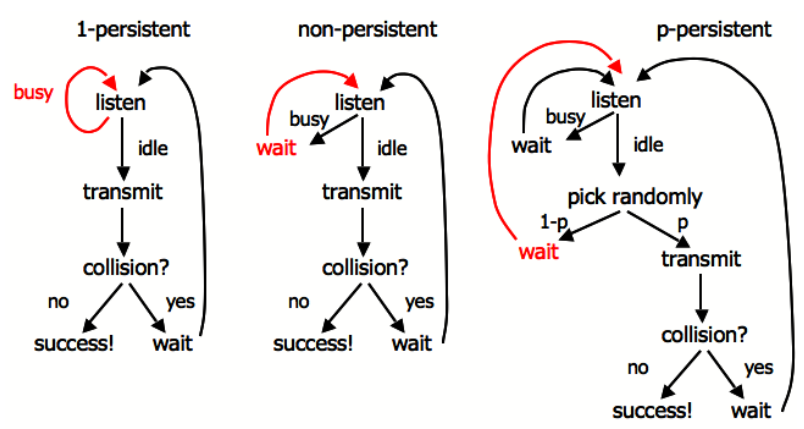
\includegraphics[width=\textwidth]{persistent}
  
  \newpage\item Collision-Free \& Limited Contention Protocols (4.2.3, 4.2.4)
    \begin{enumerate}
      \item Collision Free Protocols
        \begin{enumerate}
          \item Bit Map Protocol
            \begin{itemize}
              \item 1 bit per station overhead
              \item Division of transmission right, and transmission event
              \item Reservation based protocol
            \end{itemize}
          \item Binary Countdown Protocol
            \begin{itemize}
              \item\red{Avoid} the 1 bit per station scalability problem by using binary station addressing
              \item No collision as higher-order bit positions are used to arbitrate
              \item \textit{ATTENTION}: As soon as a station sees that a high-order bit position that is 0 in its address has been overwritten with a 1, it gives up
            \end{itemize}
          \item Token Passing
            \begin{itemize}
              \item Pass a small message called token from one station to the next in the same predefined order.
              \item In a \red{token ring} protocol, the topology of the network is used to define the order in which stations send.
            \end{itemize}
        \end{enumerate}
      \item Limited Contention Protocols
        \begin{enumerate}
          \item Adaptive Tree Walk Protocol
            \begin{itemize}
              \item All stations compete for right to transmit, if a collision occurs, binary division is used to resolve contention
              \item Tree divides stations into groups (nodes) to poll
                \begin{itemize}
                  \item Depth first search under nodes with poll collisions
                  \item Start search at lower levels ($log_2 n$) if $>1$ station expected
                \end{itemize}
              \item Illustrated
                \newline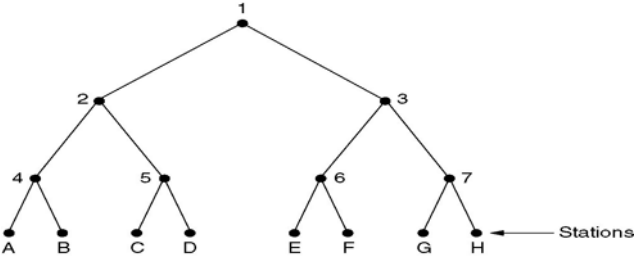
\includegraphics[width=\textwidth]{adaptivetree}
            \end{itemize}
        \end{enumerate}
    \end{enumerate}
    
  \item Wireless Protocols (4.2.5)
    \begin{enumerate}
      \item Two Problems
        \newline \red{Hidden terminal}, \red{Exposed terminal}
        \newline IDEAL CASE:
        \begin{enumerate}
          \item B wants to send to A
            \newline $ A \Leftarrow (RTS)B(RTS) \Rightarrow C\ D $
          \item C has to wait at least until B receives CTS
            \newline $ A(CTS) \Rightarrow B\ C\ D $
          \item B starts transmitting, C didn't receive any CTS after timeout duration. Then C wants to send to D so an RTS is sent by C
            \newline $ A \Leftarrow B \nRightarrow \nLeftarrow (RTS)C(RTS) \Rightarrow D $
          \item D replies
            \newline $ A\ B\ C \Leftarrow (CTS)D $
        \end{enumerate}
      \item MACA (Multiple Access with Collision Avoidance)
        \begin{enumerate}
          \item Sender asks receiver to transmit short control frame
          \item Stations near receiver hear control frame
          \item Sender can then transmit data to receiver
        \end{enumerate}
      \item MACAW (MACA for Wireless)
    \end{enumerate}
  
  \item Classic Ethernet (4.3.2) (Discussion around Figure 4.15)
    \begin{enumerate}
      \item Classic Ethernet
        \begin{itemize}
          \item Each type of Ethernet has a maximum cable length per segment
          \item Multiple cable length can be connected by repeaters - a physical device which receives, amplifies and retransmits signals in both directions
        \end{itemize}
      \item Minimum Packet Size Problem
        \newline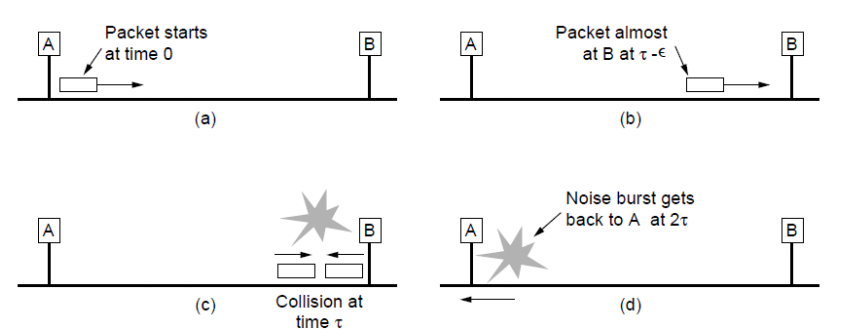
\includegraphics[width=\textwidth]{collision}
        \newline Collisions should be detected before completing the transmission of current frame
        $$ minimum\ packet = \textit{bit-rate} \times 2\tau $$
        For a 10Mbps Ethernet, typically the worst round-trip time ($2\tau$) would be nearly $50\mu sec$, so 500 bits is the smallest size. This number is rounded up to 512 bits or \red{64 bytes} for safety.
    \end{enumerate}
  
  \item Practice relevant questions from Assignment 1 and 2
\end{enumerate}

\newpage\section*{Chapter 5. The Network Layer}
\begin{enumerate}
  \item Design Goals and Store-and-Forward Packet Switching (5.1.1)
    \begin{enumerate}
      \item Design Goals
        \begin{itemize}
          \item Services should be independent of router technologies
          \item Transport layer should be shielded from number, type and topology of routers
          \item Network addressing should use a uniform numbering plan
        \end{itemize}
      \item Switching
        \newline Hosts generate packets and injects into the network, router routes packets through the network
      \item Store-and-Forward Switching \& Cut-Through Switching
        \newline (Dupe!) When the intermediate nodes receive a message in full before sending it on to the next node, this is called \red{store-and-forward switching}.
        \newline The alternative, in which the onward transmission of a message at a node starts before it is completely received by the node, is called \red{cut-through switching}.
    \end{enumerate}
    
  \item Routing Algorithms (5.2)
    \begin{enumerate}
      \item Definition
        \newline The routing algorithm is responsible for deciding on which output line an incoming packet should be transmitted.
      \item Non-Adaptive Algorithms
        \begin{enumerate}
          \item Algorithms Based on Optimality Principle
            \begin{enumerate}
              \item Sink Tree: Generating a spanning tree based on the topology
              \item Shortest Path Routing: Shortest path problem in dynamic programming
            \end{enumerate}
          \item Flooding
            \begin{itemize}
              \item Every incoming packet is sent out on every outgoing line except the one on which it arrived
              \item Generates a large number of duplicated packets - inefficient
              \item Improvement: Selective Flooding
            \end{itemize}
        \end{enumerate}
      \item Adaptive Algorithms
        \begin{enumerate}
          \item Distance Vector Routing
            \begin{enumerate}
              \item Known
                \newline\red{Best known distance} to \red{each} destination (a metric) and which line to used to get there
              \item Send to
                \newline\red{Neighbouring routers}
              \item \red{Global information shared locally}
            \end{enumerate}
          \item Link State Routing
            \begin{enumerate}
              \item Known
                \newline\red{Distance to each neighbour}
              \item Send to
                \newline\red{All other routers}
              \item \red{Local information shared globally}
            \end{enumerate}
        \end{enumerate}
      \item Hierarchical Routing
        \newline Dividing all routers into regions allows efficiencies
      \item Broadcast Routing
        \newline Allows hosts to send messages to many or all other hosts
      \item Multicast Routing
        \newline Used to send a message to a well-defined group within the whole network
        \newline Uses spanning tree to eliminate lines which do not lead to members of the group
      \item Internetwork Routing
        \begin{itemize}
          \item Within a network using an interior gateway protocol (e.g., OSPF)
          \item Between networks using an exterior gateway protocol (e.g., BGP)
        \end{itemize}
    \end{enumerate}
  
  \item Virtual Circuits (5.1.3)
    \newline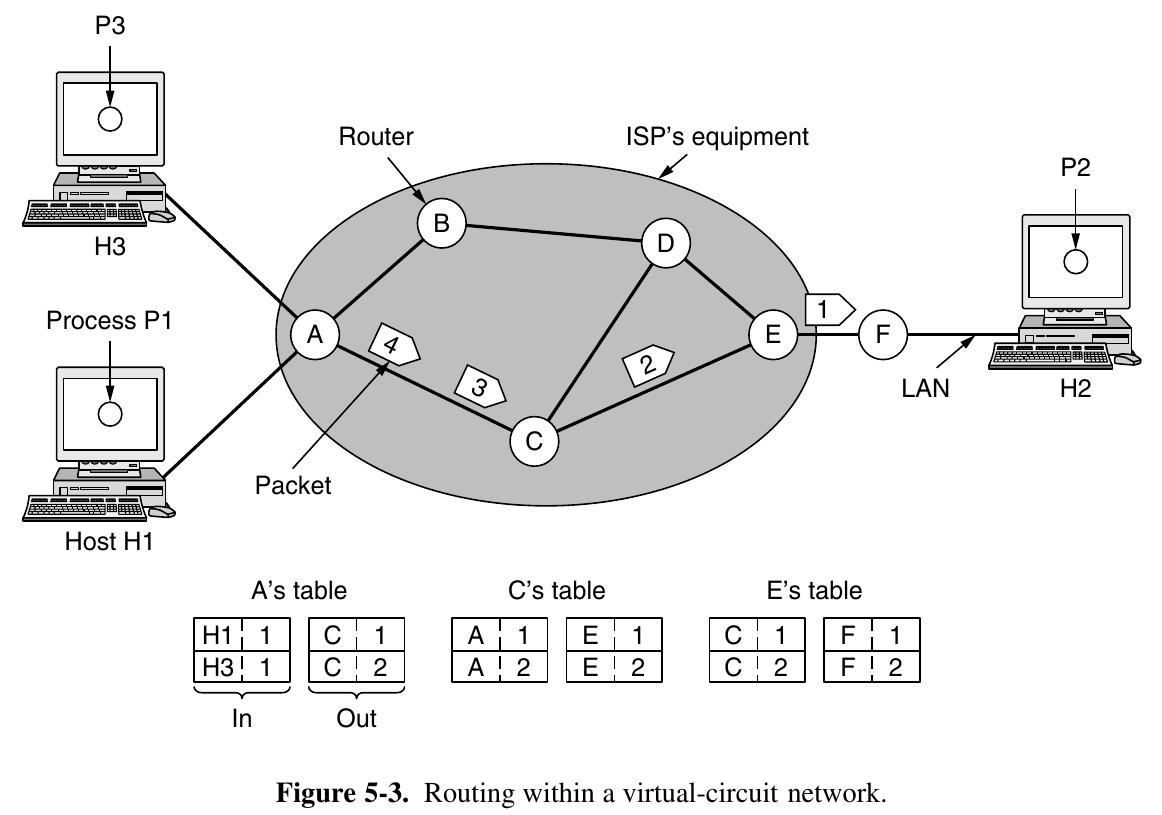
\includegraphics[width=\textwidth]{vc}
    \begin{enumerate}
    \item Definition
      \newline If connection-oriented service is used, a path from the source router all the way to the destination router must be established before any data packets can be sent. This connection is called a \red{VC (virtual circuit)} and the network is called a \red{virtual-circuit network}.
    \item\textit{ALSO CHECK}
      \begin{itemize}
        \item How to update a routing table when new info comes in
        \item Datagram routing
      \end{itemize}
    \newpage\item\textit{DIFFERENCES BETWEEN VC AND DATAGRAM}
      \begin{table}[h]\begin{tabularx}{\textwidth}{l | X | X}
        & Datagram & Virtual-Circuit \\ \hline
        Circuit setup & Not needed & required \\ \hline
        Addressing & Each packet contains the full source and destination address & Each packet contains a short VC number \\ \hline
        State Information & Routers do not hold state information about connections & Each VC requires router table space per connection \\ \hline
        Routing & Each packet is routed independently & Route chosen when VC is set up, all packets follow it \\ \hline
        Effect of router failures & None, except for packets lost during the crash & All VCs that passed through the failed router are terminated \\ \hline
        Quality of Service & Difficult & Easy if enough resources can be allocated for each VC \\ \hline
        Congestion control & Difficult & Easy if enough resources can be allocated for each VC
      \end{tabularx}\end{table}
    \end{enumerate}
  
  \item IP Protocol and IPv4 Structure (5.6.1)
    \newline Internet Protocol
    \begin{enumerate}
      \item Provides a ``best-effort'' service to route datagrams from source host to destination host
      \item These hosts may be: on \textit{same} network, or, on \textit{different} networks
      \item Each network is called an \red{Autonomous System (AS)}
    \end{enumerate}
    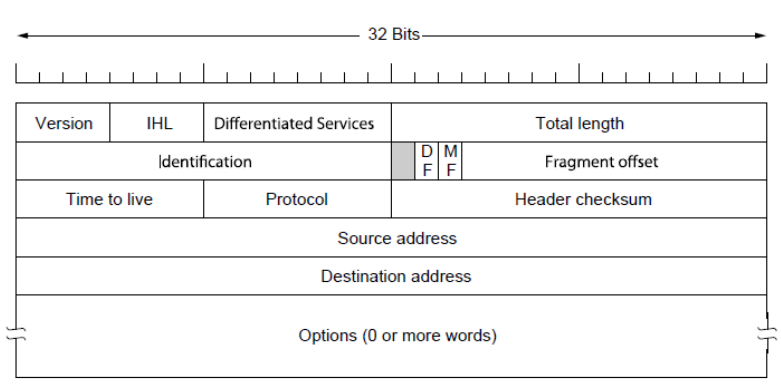
\includegraphics[width=\textwidth]{ip}
  
  \newpage\item Addressing (5.6.1, 5.6.2)
    \begin{enumerate}
      \item Classful Network
        \newline\begin{tabular}{l | r | r | r | r | r | r | l | l}
          & \specialcell{Leading\\bits} & \specialcell{Network\\bits} & \specialcell{Rest\\bits} & \specialcell{Num of\\networks} & \specialcell{Addresses\\per\\network} & \specialcell{Total\\addresses} & Start & End \\ \hline
          A & 0 & 8 & 24 & $2^7$ & $2^{24}$ & $2^{31}$ & 0.0.0.0 & 127.255.255.255 \\ \hline
          B & 10 & 16 & 16 & $2^{14}$ & $2^{16}$ & $2^{30}$ & 128.0.0.0 & 191.255.255.255 \\ \hline
          C & 110 & 24 & 8 & $2^{21}$ & $2^8$ & $2^{29}$ & 192.0.0.0 & 223.255.255.255 \\ \hline
          D & 1110 & N/D & N/D & N/D & N/D & $2^{28}$ & 224.0.0.0 & 239.255.255.255 \\ \hline
          E & 1111 & N/D & N/D & N/D & N/D & $2^{28}$ & 240.0.0.0 & 255.255.255.255
        \end{tabular}
      \item Longest Matching Prefix
        \newline Packet are forwarded to the entry with the \red{longest matching prefix} or smallest address block.
    \end{enumerate}
  
  \item ARP, RARP (5.6.4)
    \begin{enumerate}
      \item ARP (Address Resolution Protocol) finds Ethernet address of a local IP address
        \begin{itemize}
          \item Glue that is needed to send any IP packets
          \item Host queries an address and owner replies
        \end{itemize}
      \item RARP (Reverse Address Resolution Protocol)
    \end{enumerate}
  
  \item Congestion Control (5.3)
    \begin{enumerate}
      \item Definition
        \newline Too many packets present in (a part of) the network causes delay and loss that degrades performance. This situation is called \red{congestion}.
      \item Congestion Control Algorithms
        \newline Handling congestion is the responsibility of the \red{Network} and \red{Transport} layers working together
        \newline Goodput is the rate at which \textit{useful} packets are delivered by the network
        \newline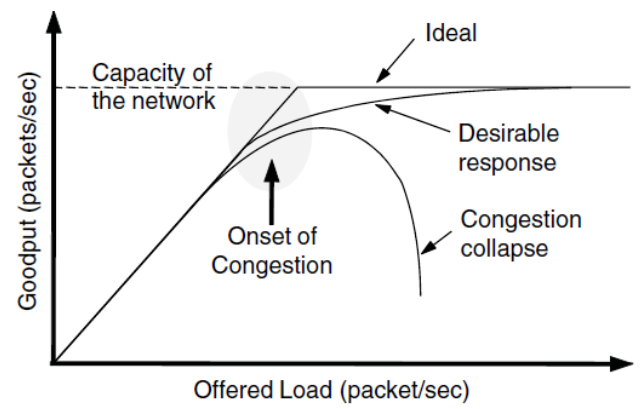
\includegraphics[width=\textwidth]{congestion}
      \item Congestion Control vs Flow Control
        \begin{itemize}
          \item \red{Flow control} is an issue for \textit{point to point} traffic, primarily concerned with preventing sender transmitting data faster than receiver can receive it
          \item \red{Congestion control} is an issue affecting the ability of the subnet to actually carry the available traffic, in a \textit{global} context
        \end{itemize}
    \end{enumerate}
\end{enumerate}

\newpage\section*{Chapter 6. The Transport Layer}
\begin{enumerate}
  \item Transport Service (6.1.1, 6.1.2)
    \begin{enumerate}
      \item Primary Function
        \newline Provide reliable cost-effective data transport from source to destination, independent of physical or data networks
      \item Layer Services
        \begin{enumerate}
          \item Definition
            \newline Transport Layer \red{Services} provide interfaces between the Application Layer and the Network Layer
          \item Transport Entities
            \begin{enumerate}
              \item Definition
                \newline Transport \red{Entities} is the hardware or software which actually does the work
              \item Location
                \begin{itemize}
                  \item OS kernel
                  \item User process
                  \item System library
                  \item NIC
                \end{itemize}
            \end{enumerate}
          \item Services
            \begin{enumerate}
              \item Purpose
                \newline Transport layer adds \red{reliability} to the Network Layer
              \item Connectionless Service (e.g., UDP)
              \item Connection-oriented Service (e.g., TCP)
            \end{enumerate}
        \end{enumerate}
      \item\textit{DIFFERENCES BETWEEN TRANSPORT LAYER AND NETWORK LAYER SERVICES}
        \begin{itemize}
          \item Transport layer code runs entirely on \red{hosts}
          \item Network layer code runs almost entirely on \red{routers}
          \item Transport layer can fix reliability problems caused by the Network Layer (e.g., delayed, lost or duplicated packets)
        \end{itemize}
      \item Role of the Transport Layer
        \begin{itemize}
          \item Providers of reliable data transmission service
            \newline at the network, data and physical layers
          \item Users of reliable data transmission services
            \newline at the application and session layers
        \end{itemize}
      \item QoS (Feature of Transport Layer)
        \begin{itemize}
          \item Reliability at application level through interface with network layer
          \item Provide a \red{simpler API} for application developers independent of network layer
        \end{itemize}
      \item Encapsulation
        \begin{enumerate}
          \item Unit
            \newline Encapsulation of \red{TPDUs} (transport layer units) in \red{packets} (network layer units) in frames (data layer units)
          \item Model
            \newline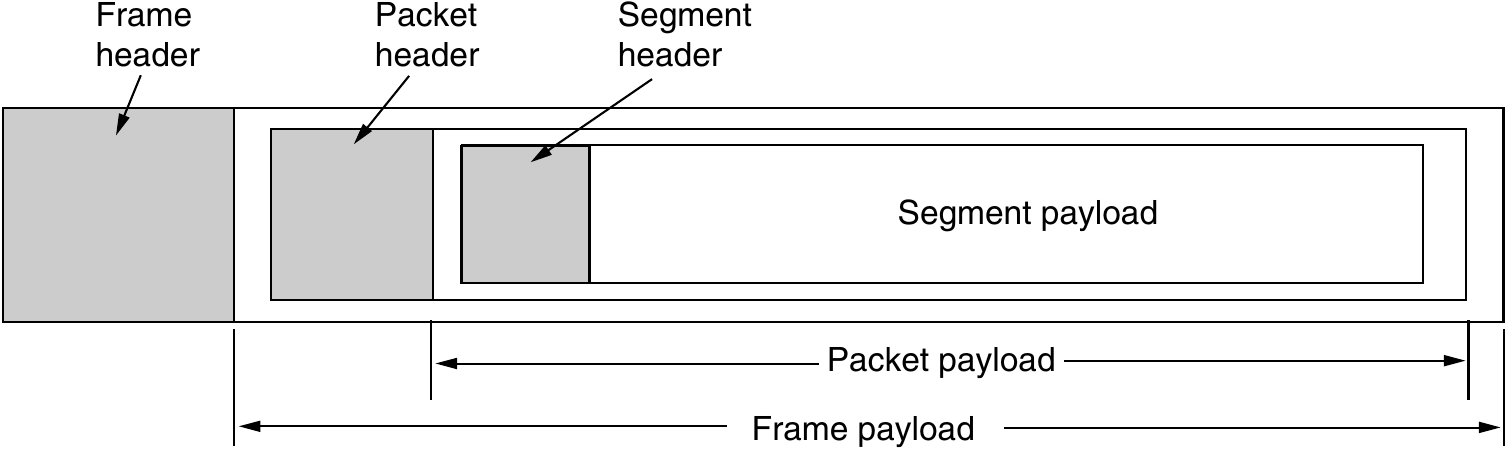
\includegraphics[width=\textwidth]{tpdu}
        \end{enumerate}
    \end{enumerate}

  \item Transport Primitives (6.1.3)
    \begin{enumerate}
      \item In a Simple Connection-Oriented Service
        \begin{enumerate}
          \item Server - \red{\texttt{LISTEN}}
          \item Client - \red{\texttt{CONNECT}}
            \begin{itemize}
              \item Sends \texttt{CONNECTION REQUEST} TPDU to Server
              \item Receives \texttt{CONNECTION ACCEPTED} TPDU from Server
            \end{itemize}
          \item Data exchanged using \red{\texttt{SEND}} and \red{\texttt{RECEIVE}}
          \item Either party - \red{\texttt{DISCONNECT}}
        \end{enumerate}
      \item Disconnect Primitives
        \begin{enumerate}
          \item Asymmetric Disconnection
            \begin{itemize}
              \item Either party can issue a \texttt{DISCONNECT}, which results in
              \item \texttt{DISCONNECT} TPDU and transmission ends in both directions
            \end{itemize}
          \item Symmetric Disconnect
            \begin{itemize}
              \item Both parties issue \texttt{DISCONNECT}
              \item Closing only one direction at a time - allows flexibility to remain in receive mode
            \end{itemize}
        \end{enumerate}
    \end{enumerate}

  \item Connection Establishment (3-way handshake) (6.2.2)
    \begin{enumerate}
      \item Issues
        \newline Packets may be lost, corrupted, \red{delayed}, and \red{duplicated}
      \item Solutions
        \begin{itemize}
          \item Don't reuse \red{Maximum Segment Lifetime} sequence numbers
          \item Three-way handshake for establishing connection
          \item Use a sequence number space large enough that it will not wrap, even when sending at full rate
        \end{itemize}
      \item Three-Way Handshake
        \begin{enumerate}
          \item Principle
            \newline Sender and receivers exchange information about which sequencing strategy each will use, and agree on it before transmitting TPDU's
          \item Model
            \newline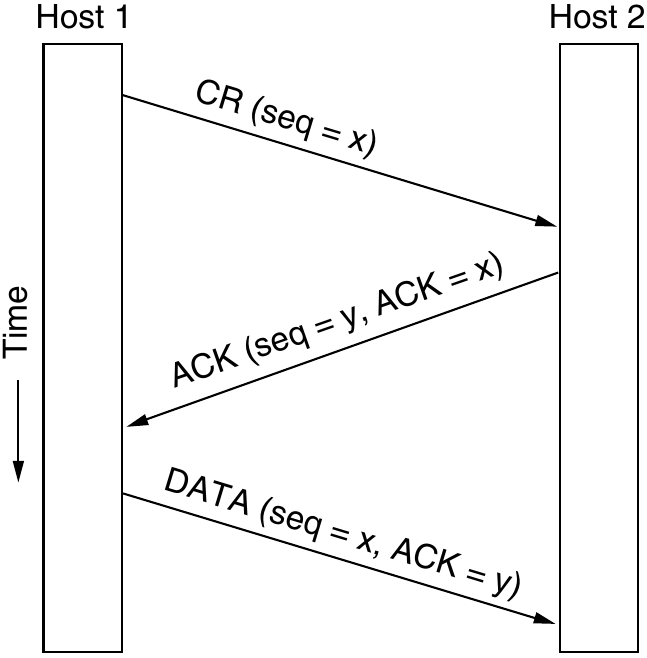
\includegraphics[width=0.50\textwidth]{3way}
            \newline CR = Connection Request
        \end{enumerate}
    \end{enumerate}

  \item Connection Release (6.2.3)
    \begin{enumerate}
      \item Issues
        \begin{itemize}
          \item Asymmetric release may result in data lose hence symmetric release is more attractive
          \item Symmetric release works well were each process has a set amount of data to transmit and knows when it has been sent
        \end{itemize}
      \item Solutions
        \begin{itemize}
          \item Three-way handshake
          \item Finite retry
          \item Timeouts
        \end{itemize}
      \item Three-Way Handshake
        \newline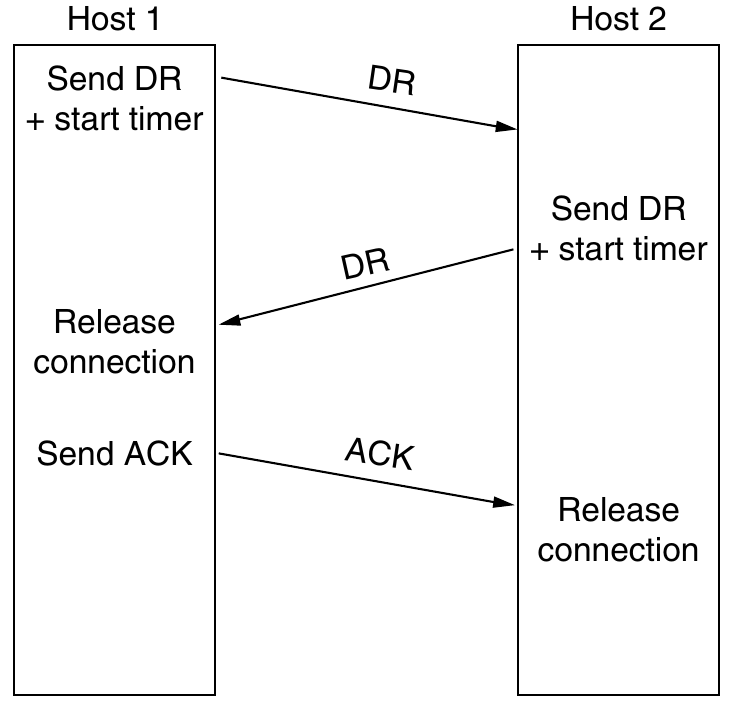
\includegraphics[width=0.50\textwidth]{3wayrelease}
        \newline DR = Disconnect Request (both DRs are ACKed by the other side)
    \end{enumerate}

  \item User Datagram Protocol (UDP) (6.4.1)
    \begin{enumerate}
      \item Advantage
        \newline Main \red{advantage} of using UDP over raw IP is the ability to specify ports for source and destination pairs (and both ports are required)
      \item Strengths and Weaknesses
        \begin{enumerate}
          \item Strengths
            \newline Provides an IP interface with multiplexing/demultiplexing capabilities and consequently, transmission efficiencies
          \item Weaknesses
            \newline UDP does not include support for flow control, error control or retransmission of bad segments
          \item\red{Conclusion}
            \newline Where applications don't require a precise level of control over packet flow/error/timing, UDP is a good choice
        \end{enumerate}
    \end{enumerate}

  \item Remote Procedure Call (RPC) Using UDP (6.4.2)
    \begin{enumerate}
      \item Definition
        \newline Sending a message and getting a reply back is analogous to making \red{a function call} in programming languages
      \item Principle
        \begin{itemize}
          \item To call a remote procedure, the client is bound to a small library (the \red{client stub}) that represents the server procedure in the client's address space
          \item Similarly the server is bound with a procedure called the \red{server stub}. These stubs hide the fact that the procedure itself is not local
          \item UDP with \red{retransmission} is low-latency transport
        \end{itemize}
    \end{enumerate}

  \item Transmission Control Protocol (TCP) (6.5.1)
    \begin{enumerate}
      \item Purpose
        \newline Provides a protocol by which applications can transmit IP datagrams within a \red{connection-oriented} framework, thus increasing reliability
      \item Location of Entities
        \begin{itemize}
          \item Kernel
          \item Library
          \item User process
        \end{itemize}
      \item Service Model
        \begin{itemize}
          \item Sender and receiver both create Berkeley sockets on specific IP addresses
          \item Connections must be explicitly established between sockets at sending and receiving hosts
          \item A socket may be used for multiple connections simultaneously
        \end{itemize}
      \item Feature
        \begin{itemize}
          \item \red{Full duplex} - data in both directions simultaneously
          \item \red{Point to point} - exact pair of senders and receivers
          \item \red{Byte streams}, not message streams - message boundaries are not preserved
          \item \red{Buffer capable} - TCP entity can choose to buffer prior to sending or not depending on the contest
            \begin{itemize}
              \item \texttt{PUSH} flag - indicates a transmission not to be delayed
              \item \texttt{URGENT} flag - indicates that transmission should be send immediately
            \end{itemize}
        \end{itemize}
      \item Characteristics
        \begin{enumerate}
          \item Unit: Segment
          \item Header: fixed 20 byte header plus zero or more data types
          \item Segment Size Decision Policy
            \begin{itemize}
              \item 65,515 byte IP payload
              \item Maximum Transfer Unit (MTU) - generally 1500 bytes
            \end{itemize}
          \item \red{Sliding window protocol}
        \end{enumerate}
      \item Connection Establishment and Release
        \begin{enumerate}
          \item Connections established using \red{three-way handshake}
          \item Two simultaneous connection attempts results in only one connection (uniquely identified by end points)
          \item Connections released asynchronously (2 $\times$ asymmetric releases, one for each transmission direction)
          \item Timers used to lost connection releases (three army problem)
        \end{enumerate}
      \item Transmission Policy
        \begin{itemize}
          \item TCP acknowledges bytes, not packets
          \item Receiver advertises window based on avail buffer space
        \end{itemize}
    \end{enumerate}

  \item TCP Congestion Control (6.5.9)
  \begin{enumerate}
    \item Significance
      \newline Although lower layers (data and network) attempt to ameliorate congestion, in reality TCP impacts congestion most significantly because TCP offers methods to transparently reduce the data rate, and hence reduce congestion itself
    \item Issues
      \begin{itemize}
        \item \red{Network capacity} and \red{receiver capacity}
        \item Should be dealt with separately, but compatibly
      \end{itemize}
    \item Solution
      \newline Sender maintains two windows
      \begin{itemize}
        \item \red{Window} described by the \red{receiver}
        \item \red{Congestion window}
      \end{itemize}
    \item Congestion Window
      \begin{itemize}
        \item After connection is established, sender initializes congestion window to \red{maximum size of segment}
        \item\[
                cwnd(i) =
                  \begin{cases}
                    max\ segment,               & i = 0 \\
                    cwnd(i-1)\times 2,          & cwnd(i-1) < thr \text{ and } cwnd(i) < thr \\
                    thr,                        & cwnd(i-1) < thr \text{ and } cwnd(i) \geq thr \\
                    cwnd(i-1) + max\ segment,   & cwnd(i-1) \geq thr
                  \end{cases}
             \]
             $$ thr\textit{ (threshold) } = \frac{previous\ loss\ cwnd}{2} $$
        \item Illustrated Increment of Congestion Window
          \newline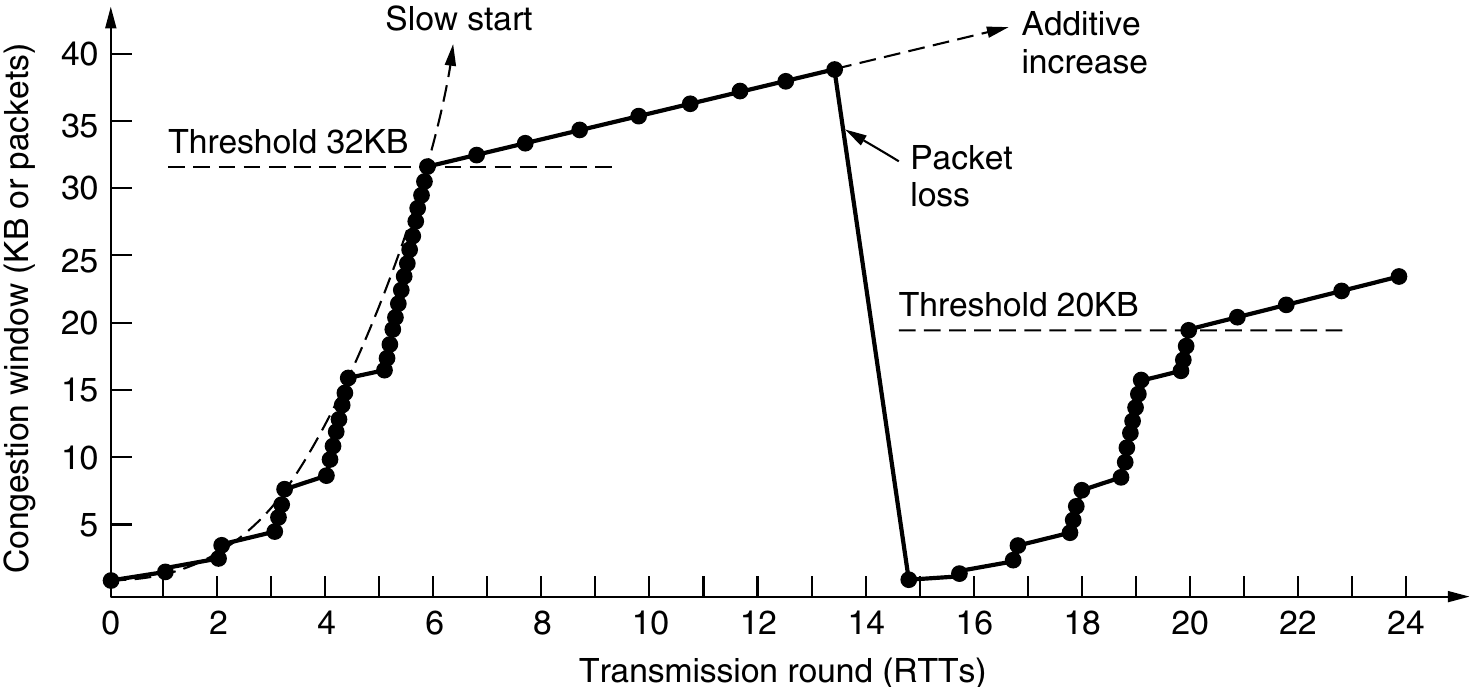
\includegraphics[width=\textwidth]{congestionwindow}
      \end{itemize}
  \end{enumerate}
\end{enumerate}

\newpage\section*{Chapter 7. The Application Layer}
\begin{enumerate}
  \item Domain Name System (DNS) (7.1)
    \begin{enumerate}
      \item Definition
        \begin{itemize}
          \item \red{Distributed database} implemented in hierarchy of many \red{name servers}
          \item \red{Application-layer protocol} that allows a host to query the database in order to \red{resolve} names (address/name translation)
          \item used by other application-layer protocols (HTTP, FTP, SMTP)
        \end{itemize}
      \item Resource Records
        \begin{enumerate}
          \item Definition
            \newline Every domain, whether it is a single host or a top-level domain, can have a set of \red{resource records} associated with it. These records are the \red{DNS database}.
          \item Structure
            \newline A resource record is a five-tuple:
            \newline\begin{itemize*}
              \item [] Domain\_name
              \item [] Time\_to\_live
              \item [] Class
              \item [] Type
              \item [] Value
            \end{itemize*}
          \item Explanation of Fields
            \begin{enumerate}
              \item Domain\_name
                \newline The \textit{Domain\_name} tells the domain to which this record applies. Normally, many records exist for each domain and each copy of the database holds information about multiple domains. The order of the records is not significant.
              \item Time\_to\_live
                \newline The \textit{Time\_to\_live} field gives an indication of how stable the record is. (Unit: second)
              \item Class
                \newline For Internet information, it is always \textit{IN}. For non-Internet information, other codes can be used, but rarely seen.
              \item Type
                \newline The \textit{Type} field tells what kind of record this is.
            \end{enumerate}
          \item Type List
            \newline\begin{tabular}{l | l | l}
              Type & Meaning & Value \\ \hline
              SOA & Start of authority & Parameters for this zone \\ \hline
              \red{A} & IPv4 address of a host & 32-Bit integer \\ \hline
              \red{AAAA} & IPv6 address of a host & 128-Bit integer \\ \hline
              \red{MX} & Mail exchange & Priority, domain willing to accept email \\ \hline
              NS & Name server & Name of a server for this domain \\ \hline
              \red{CNAME} & Canonical name & Domain name \\ \hline
              PTR & Pointer & Alias for an IP address \\ \hline
              SPF & Sender policy framework & Text encoding of mail sending policy \\ \hline
              SRV & Service & Host that provides it \\ \hline
              TXT & Text & Descriptive ASCII text
            \end{tabular}
        \end{enumerate}
      \item DNS Resolution
        \begin{enumerate}
          \item Definition
            \newline Finding the IP address for a given hostname is called \red{resolution} and is done with the DNS protocol
          \item Principle
            \begin{itemize}
              \item Computer requests local name server to resolve
              \item Local name server asks the root name server
              \item Root returns the name server for a lower zone
              \item Continue down zones until name server can answer
            \end{itemize}
          \item Recursive Query \& Iterated Query
            \begin{enumerate}
              \item Recursive Query
                \newline The local name server handles the resolution on behalf of the host which is querying, until it has the desired answer to return. It does \textit{not} return partial answers.
              \item Iterated Query
                \newline The root name server (and each subsequent name server) does \textit{not} recursively continue the query for the local name server. It just returns a partial answer and moves on to the next query. The local name server is responsible for continuing the resolution by issuing further queries.
              \item Example
                \newline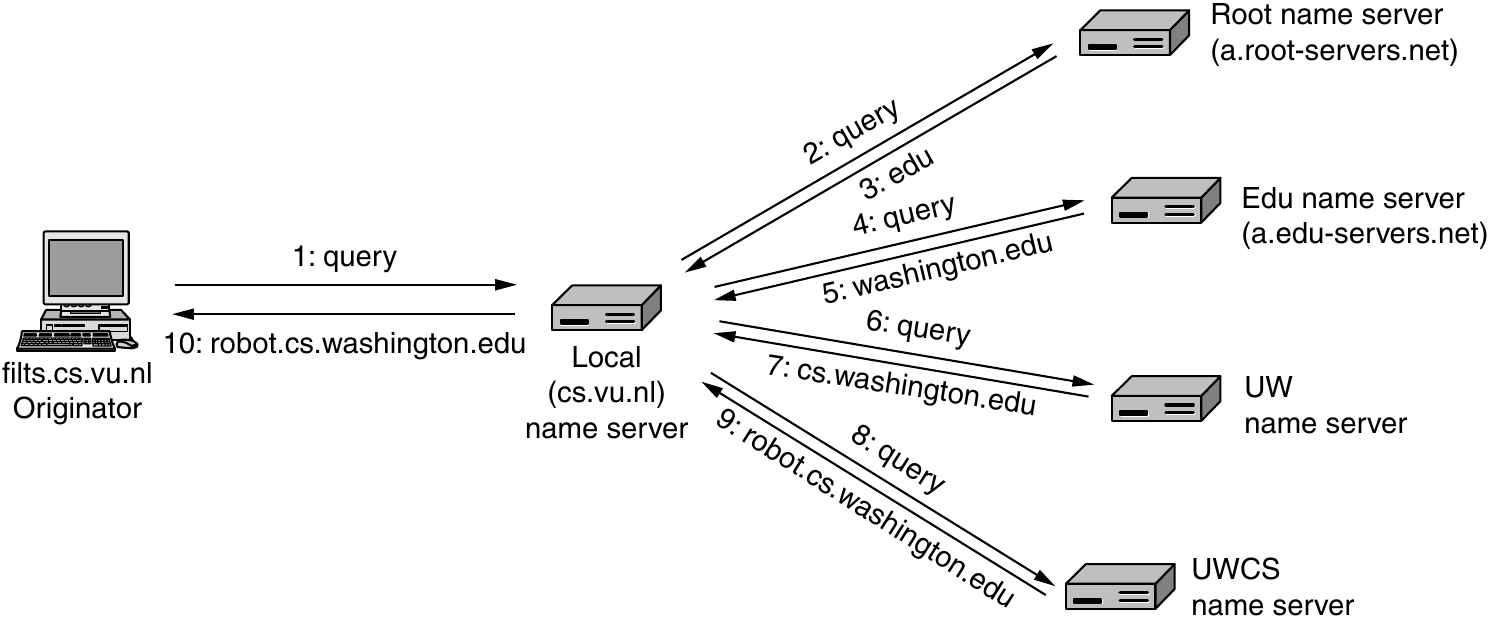
\includegraphics[width=\textwidth]{dns}
            \end{enumerate}
        \end{enumerate}
      \item DNS Protocol
        \begin{itemize}
          \item Runs on UDP port 53, retransmits lost messages
          \item Caches name server answers for better performance
        \end{itemize}
    \end{enumerate}

  \item Email (7.2)
    \begin{enumerate}
      \item Architecture and Services (7.2.1)
        \begin{enumerate}
          \item Architecture \& Components
            \begin{enumerate}
              \item User Agents
                \newline Allow people to read and send email
              \item Mail Servers (Message Transfer Agents)
                \newline Move the messages from the source to the destination
              \item Simple Mail Transfer Protocol (SMTP)
                \newline SMTP is used to send messages from the sender's
                \begin{itemize}
                  \item \textit{mail server} to the receiver's \textit{mail server}
                  \item \textit{user agent} to the sender's \textit{mail server}
                \end{itemize}
              \item Illustrated Architecture
                \newline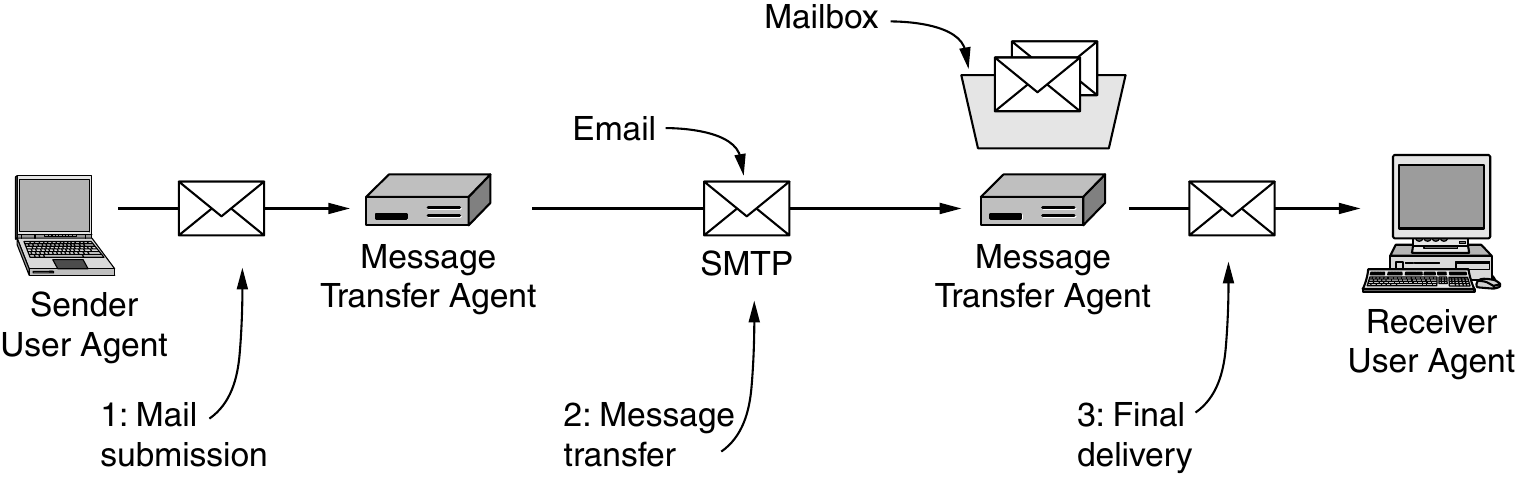
\includegraphics[width=\textwidth]{emailsystem}
            \end{enumerate}
          \item Services
            \begin{enumerate}
              \item Mail Submission
                \newline Sending new messages into the mail system for delivery.
              \item Mailing List
                \newline Message transfer agents (mail servers) implement mailing lists, in which an identical copy of a message is delivered to everyone on a list of email addresses.
              \item Mailboxes
                \newline Mailboxes store the email that is received for a user.
            \end{enumerate}
        \end{enumerate}

      \item Comparison: POP3 and IMAP (7.2.5)
        \begin{enumerate}
          \item Internet Message Access Protocol (IMAP)
            \begin{itemize}
              \item Addressing mail by using attributes
              \item Search can be performed on server to find messages that satisfy certain criteria so that only those messages are fetched by the client
            \end{itemize}
          \item Post Office Protocol, version 3 (POP3)
            \begin{itemize}
              \item Less secure
              \item Mail is downloaded to the user agent computer, instead of remaining on the mail server
                \begin{itemize}
                  \item Easier for servers
                  \item Not easy to read mail on multiple computers
                  \item Risk of losing mail
                \end{itemize}
            \end{itemize}
        \end{enumerate}
    \end{enumerate}
  \item WWW (7.3)
    \begin{enumerate}
      \item Architecture (7.3.1)
        \begin{enumerate}
          \item Client - Server Model
            \begin{itemize}
              \item Client - Browser based access to pages
              \item Server - Daemon based content delivery of pages
              \item Uniform Resource Locator (URL)
                \begin{itemize}
                  \item Protocol + DNS Name + file name
                  \item Extensions of URL - URN (location independent)
                \end{itemize}
            \end{itemize}
          \item Pages are named with URLs
          \item Illustrated Architecture
            \newline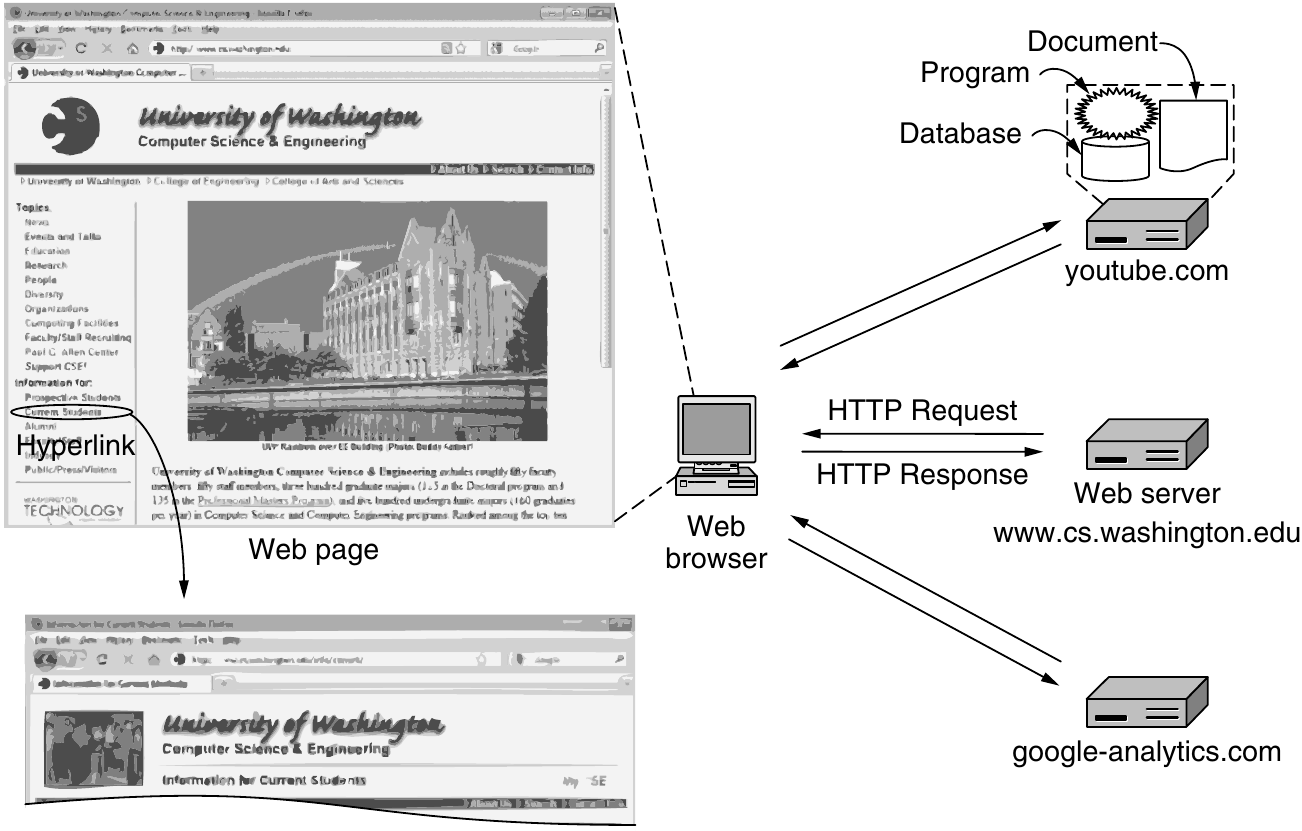
\includegraphics[width=\textwidth]{www}
        \end{enumerate}
      \item Hypertext Transfer Protocol (HTTP) (7.3.4)
        \begin{enumerate}
          \item Connections
            \begin{itemize}
              \item [HTTP 1.0] \red{Single} connect for each transaction for each client-server pair
              \item [HTTP 1.1] \red{Persistent} connections per server-client pair
            \end{itemize}
          \item Methods
            \begin{itemize}
              \item [\red{GET}] Request to read a Web page
              \item [HEAD] Request to read a Web page's header
              \item [\red{PUT}] Request to store a Web page
              \item [\red{POST}] Append to a named resource (e.g., a Web page)
              \item [DELETE] Remove the Web page
              \item [TRACE] Echo the incoming request
              \item [CONNECT] Reserved for future use
              \item [OPTIONS] Query certain options
            \end{itemize}
          \item Error Codes
            \newline\begin{tabular}{c | l | l}
              Code & Meaning & Examples \\ \hline
              1xx & Information & 100=server agrees to handle client's request \\
              2xx & Success & 200=request succeeded; 204=no content present \\
              3xx & Redirection & 301=page moved; 304=cache page still valid \\
              4xx & Client Error & 403=forbidden page; 404=page not found \\
              5xx & Server Error & 500=internal server error; 503=try again later
            \end{tabular}
        \end{enumerate}
    \end{enumerate}
    
  \item Multimedia Networks (7.4)
    \begin{enumerate}
      \item Basic Model and Characteristics (7.4.3)
        \begin{enumerate}
          \item Step by Step
            \begin{itemize}
              \item [Step 0] User clicks a movie
              \item [Step 1] Browser sends an HTTP request to the Web server
              \item [Step 2] The server fetches the movie and sends it back to browser with \textit{MIME} attached
              \item [Step 3] The browser saves the entire movie to a scratch file on the disk
              \item [Step 4] The media player starts reading and playing the movie
            \end{itemize}
          \item Illustrated Model
            \newline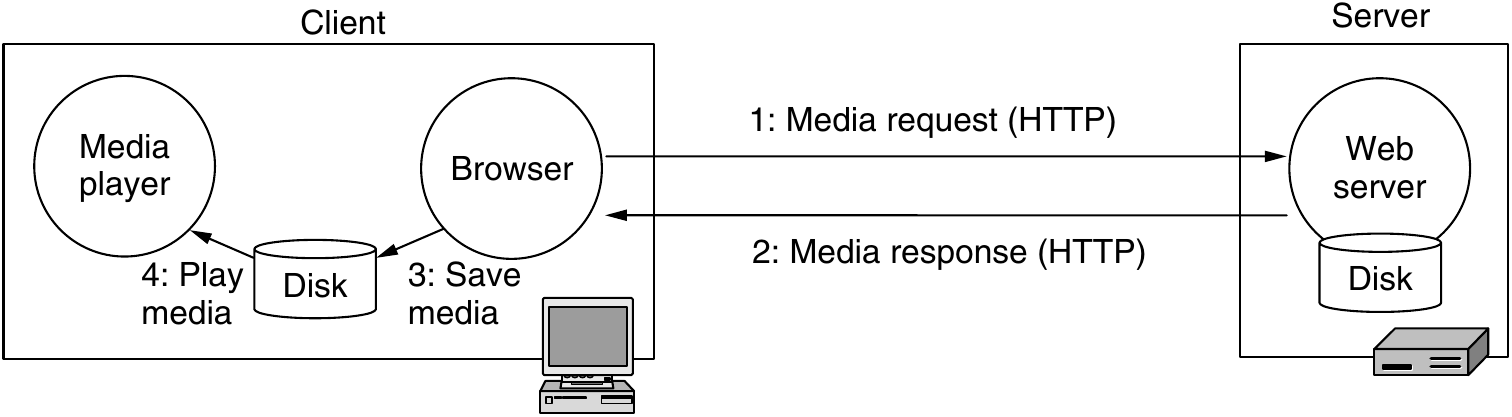
\includegraphics[width=\textwidth]{media}
          \item Characteristics
            \begin{itemize}
              \item Higher bandwidth requirements
              \item Higher QoS requirement
              \item New infrastructure models
              \item New service providers
            \end{itemize}
        \end{enumerate}
      \item Jitter Management (7.4.3)
        \begin{enumerate}
          \item Approach
            \begin{enumerate}
              \item Multimedia software \red{buffers} streamed media sources prior to transmission
              \item Buffering is a \red{defensive} mechanism to reduce jitter
              \item Ideally, the stream buffer will continue to be filled at the same rate the stream is played back to the user
            \end{enumerate}
          \item Buffering Modes
            \begin{enumerate}
              \item Pull Server
                \newline As long as there is room in the buffer to another block, the media player continues to request additional blocks from the server (goal to keep the buffer as full as possible)
              \item Push Server
                \newline Media player sends a play request, and the server continuously pushes data to the player, media player uses a FIFO (First-In First-Out) scheme to draw from the buffer, and uses a compensation mechanism when the buffer is not filled to capacity - high and low watermarks trigger starts or stops in the playback
            \end{enumerate}
          \item Push Server Mode
            \begin{enumerate}
              \item Approach
                \newline The startup delay gives the buffer a change to fill to the \red{low-water mark}, then if data are sometimes slow to arrive due to congestion, the buffered media will allow the playout to continue normally until new media arrive and the buffer is replenished.
                \newline The \red{more} jitter, the \red{larger} the low-water mark of the buffer needs to be to avoid underrun.
                \newline \red{High-water mark} is defined so that buffering too much can be avoided. Basically, the server just pumps out data until the buffer is filled to the high-water mark.
              \item Illustrated Model
                \newline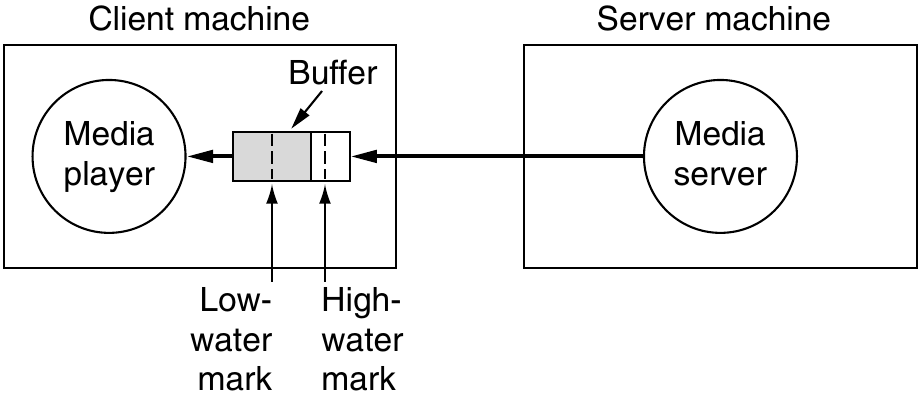
\includegraphics[width=\textwidth]{mediajitter}
            \end{enumerate}
        \end{enumerate}
    \end{enumerate}
\end{enumerate}

\newpage\section*{Chapter 8. Network Security}
\begin{enumerate}
  \item Basic Encryption (8.1.1)
    \begin{enumerate}
      \item Encryption Model
        \newline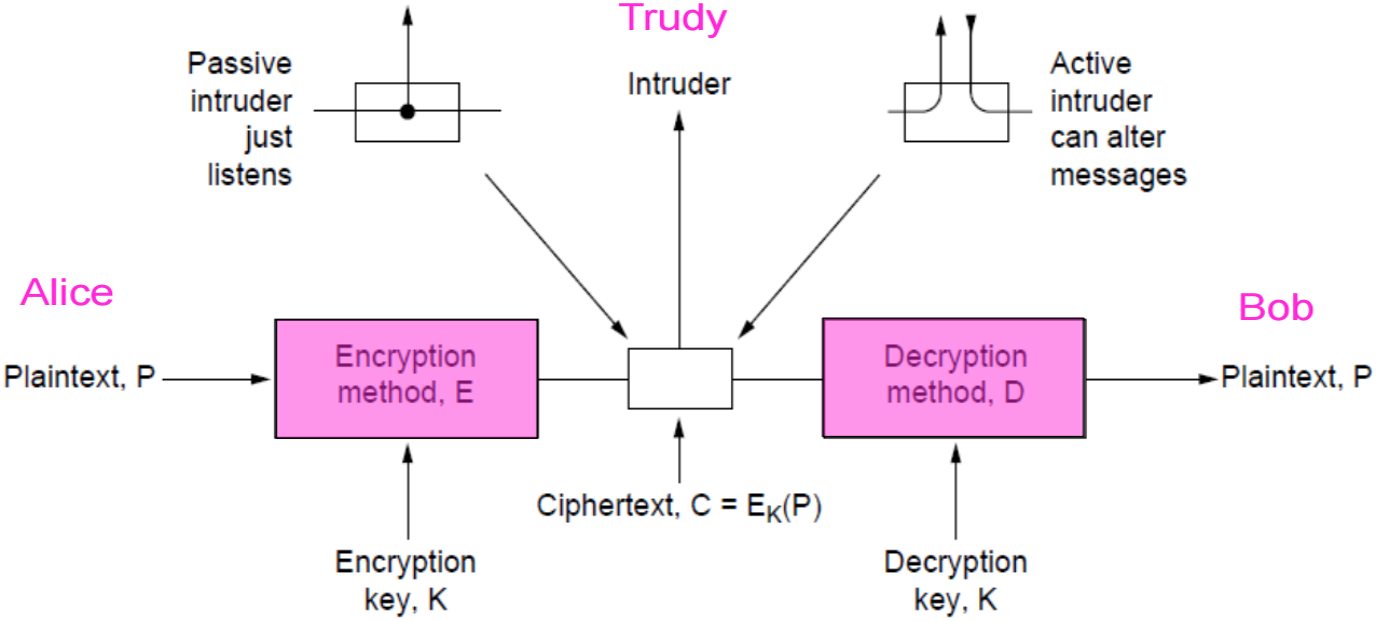
\includegraphics[width=\textwidth]{encryption}
      \item Plaintext, Keys, Ciphertext
        \newline \red{Plaintext} messages to be encrypted can be transformed (encrypted/decrypted) by a function that is parameterized by a \red{key}, the output of the transformation process is \red{ciphertext}
      \item Kerckhoff's Principle
        \newline Cryptographic Algorithms and related functions (E, D) are public; only the keys (K) are secret
      \item Relations
        \newline $ C = E_K(P) $
        \newline $ P = D_K(C) $
        \newline $ D_K(E_K(P)) = P $
        \newline Requirement: $ D_{K1}(E_{K2}(P)) = P $ if and only if $ K1 = K2 $
    \end{enumerate}
    
  \item Types of Ciphers
    \begin{enumerate}
      \item Substitution Cipher (8.1.2)
        \begin{enumerate}
          \item Definition
            \newline Each letter of group of letters is replaced systematically by other letters or groups of letters
          \item Vulnerability
            \newline Breakable with knowledge of the replacement system
        \end{enumerate}
      \item Transposition Cipher
        \begin{enumerate}
          \item Definition
            \newline All letters are re-ordered without disguising them
          \item Vulnerability
            \newline Breakable with knowledge of re-ordering system
        \end{enumerate}
      \item One-time Pad
        \begin{enumerate}
          \item Definition
            \newline Uses a random bit string as the key, convert the plaintext into a bit string, then XOR the two strings bit by bit
          \item Vulnerability
            \newline Unbreakable because given a sufficiently large sample of each letter, digram, and trigram will occur with equal distribution
        \end{enumerate}
    \end{enumerate}
    
  \item Symmetric Key Algorithms
    \begin{enumerate}
      \item Definition
        \newline Uses the \red{same key} for both encryption and decryption
      \item Ciphers Used
        \newline Symmetric key algorithms can use permutation, substitution and a combination of both to encrypt and decrypt
      \item Examples
        \begin{enumerate}
          \item Data Encryption Standard (DES)
            \begin{itemize}
              \item 64 bit blocks and 56 bit keys
              \item $ 2^{56} $ key space
              \item Triple DES has a $ 3\times 2^{56} $ key space
            \end{itemize}
          \item Advanced Encryption Standard (AES)
            \begin{itemize}
              \item 128 bit blocks and 128 bit keys (others available)
              \item $ 2^{128} $ key space
            \end{itemize}
        \end{enumerate}
      \item Cipher Modes (8.2.3)
        \begin{enumerate}
          \item Block
            \newline Replacement attack
          \item Block Chaining
            \begin{enumerate}
              \item Definition
                \newline Each plaintext block is XOR'ed with the previous ciphertext block before being encrypted
              \item Feature
                \newline If one block of ciphertext ($ C_i $) is changed before decryption, only $ P_i $ and $ P_{i+1} $ are affected
              \item Advantage
                \begin{itemize}
                  \item Random access
                  \item Anti replacement attack
                \end{itemize}
              \item Disadvantage
                \begin{itemize}
                  \item Inefficient (Can only start decrypting when 8 bytes fetched)
                  \item 1 bit error, 16 bytes error
                \end{itemize}
              \item Model
                \newline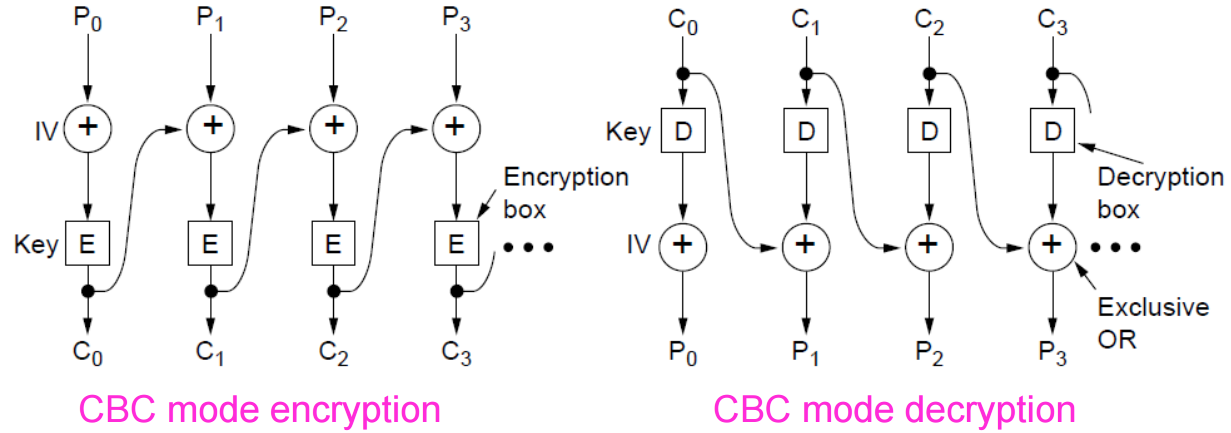
\includegraphics[width=\textwidth]{blockchaining}
            \end{enumerate}
          \item Feedback Mode
            \begin{enumerate}
              \item Definition
                \newline Byte-by-byte encryption is used rather than block-by-block encryption, together with a shift register
              \item Feature
                \begin{itemize}
                  \item If one byte of ciphertext ($ C_i $) is changed before decryption, $ P_i $ to $ P_{i+L} $ are affected ($L$ is the length of shift register in bytes)
                  \item Inefficient
                \end{itemize}
              \item Advantage
                \begin{itemize}
                  \item Be able to start decrypting when 1 byte fetched
                \end{itemize}
              \item Disadvantage
                \begin{itemize}
                  \item Inefficient (1 byte product for encrypting/decrypting 8 bytes)
                  \item 1 bit error, 9 bytes error (when 64-bit register is used)
                \end{itemize}
              \item Model
                \newline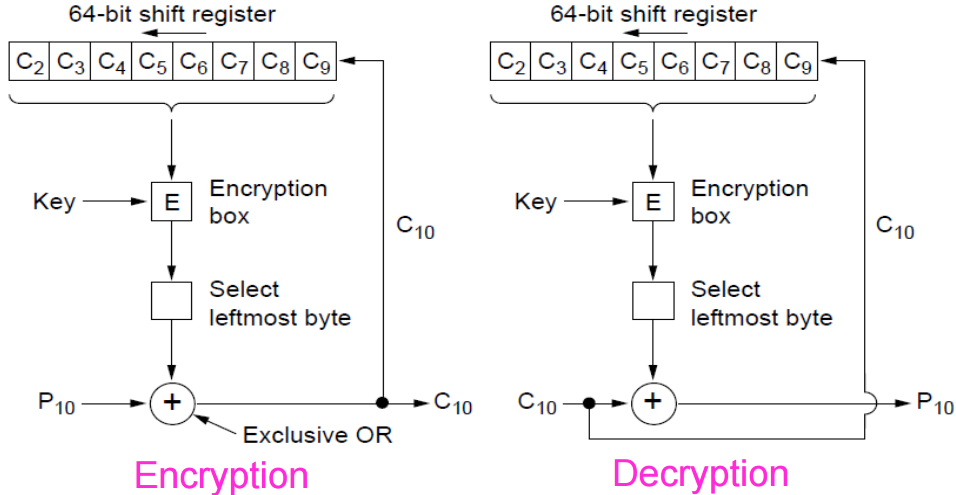
\includegraphics[width=\textwidth]{feedback}
            \end{enumerate}
          \item Stream Cipher
            \begin{enumerate}
              \item Definition
                \newline In stream cipher mode, recursive sequential block encryption is used as an one-time pad, and XOR'ed with plaintext to generate ciphertext
              \item Advantage
                \begin{itemize}
                  \item 1 bit error, 1 byte influenced
                \end{itemize}
              \item Disadvantage
                \begin{itemize}
                  \item No random access
                \end{itemize}
              \newpage\item Model
                \newline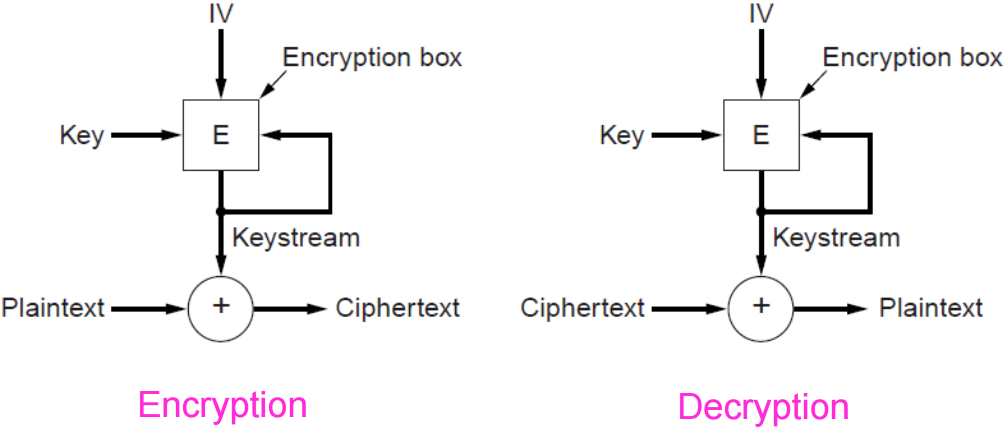
\includegraphics[width=\textwidth]{stream}
            \end{enumerate}
          \item Counter Mode
            \begin{enumerate}
              \item Definition
                \newline In counter mode, plaintext is not directly encrypted, but an initialization parameter plus an arbitrary constant is encrypted, and the resulting ciphertext is XOR'ed with plaintext to generate new
              \item Advantage
                \begin{itemize}
                  \item Random access
                \end{itemize}
              \item Disadvantage
                \begin{itemize}
                  \item Replay attack
                \end{itemize}
              \item Model
                \newline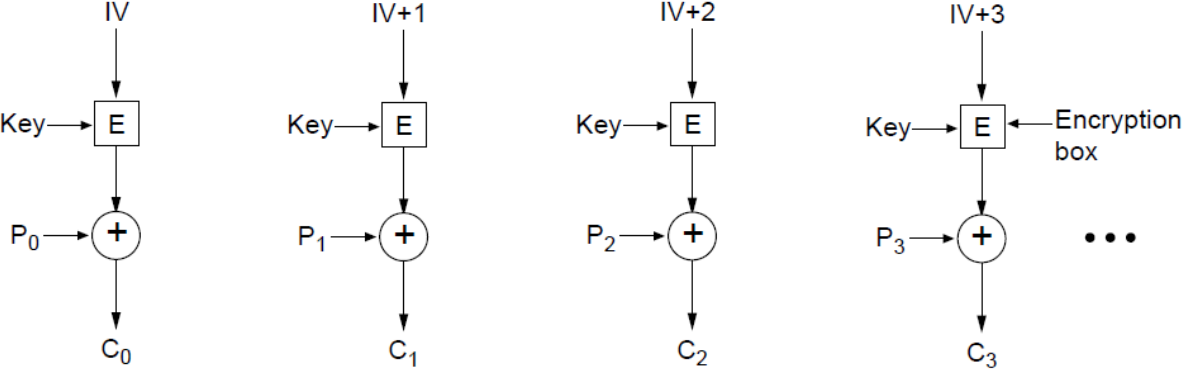
\includegraphics[width=\textwidth]{counter}
            \end{enumerate}
        \end{enumerate}
      \item Other Algorithms
        \begin{itemize}
          \item Blowfish
          \item IDEA
          \item RC4
          \item RC5
        \end{itemize}
    \end{enumerate}

  \item Asymmetric Key Algorithms
    \begin{enumerate}
      \item Definition
        \newline The key used to encrypt and the key used to decrypt are different, and not derivable from each other
      \item Public Key Algorithms (Diffie-Hellman Key Exchange)
        \begin{enumerate}
          \item 2-Key System
            \begin{itemize}
              \item [Key 1] Public key, usable by anyone to encrypt messages to the owner of the key
              \item [Key 2] Private key, required to decrypt the message (and held only by the owner of the key)
            \end{itemize}
        \end{enumerate}
      \item RSA (8.3.1)
        \begin{enumerate}
          \item Encryption \& Decryption
            \begin{itemize}
              \item [Encryption] $ Cipher = Plain^e(mod\ n) $
              \item [Decryption] $ Plain = Cipher^d(mod\ n) $
            \end{itemize}
          \item Usage
            \newline RSA is too slow for encrypting/decrypting large volumes of data, but is widely used for \red{secure key distribution}
        \end{enumerate}
      \item Digital Signatures
        \begin{enumerate}
          \item Reason of Using Cryptography
            \newline Cryptographic approaches can be used to ensure \red{authenticity} and allow for \red{non-repudiation}
          \item Requirements
            \begin{itemize}
              \item Receiver can verify the claimed identity of the sender
              \item Sender cannot repudiate contents of the message
              \item Receiver cannot have derived the message themselves
            \end{itemize}
          \item Message Digests
            \begin{enumerate}
              \item Definition
                \newline Using a one-way hash function to take an arbitrary length of plaintext and compute a fixed-length bit string
              \item Properties
                \begin{itemize}
                  \item Given $P$, it is easy to compute $\textit{MD}(P)$
                  \item Given $\textit{MD}(P)$ it is effectively impossible to find $P$
                  \item Given $P$, no one can find $P_0$ such that $\textit{MD}(P_0)=\textit{MD}(P)$
                  \item A change in even a single bit of input produces a very different output
                \end{itemize}
            \end{enumerate}
          \item Birthday Attack
            \newline $ 2^{m/2} $ may be sufficient to break a message digest algorithm
          \item Public Key Management
            \begin{enumerate}
              \item Approaches
                \begin{itemize}
                  \item Certification Authority (CA)
                    \newline A trusted intermediary who uses non-electronic identification to identify users prior to certifying keys and certificates
                  \item X.509
                    \newline An international standard for certificate expression
                  \item PKI
                    \newline Hierarchically structured certificate authorities allow for the establishment of a chain of trust or certification path
                \end{itemize}
              \item Man in the middle
                \newline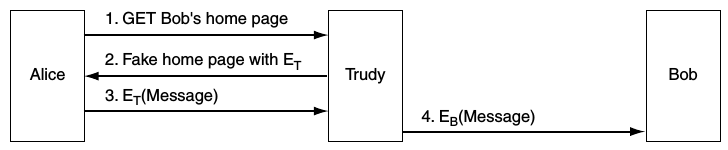
\includegraphics[width=\textwidth]{maninthemiddle}
            \end{enumerate}
        \end{enumerate}
    \end{enumerate}

  \newpage\item Communication Network Security (8.6)
    \begin{enumerate}
      \item Authentication Protocols
        \begin{enumerate}
          \item Shared Secret Key
            \begin{itemize}
              \item Principle
                \newline One party sends a random number to the other party, who transforms it and sends the result back - essentially a challenge and response protocol
              \item Identity Confirmation
                \newline A mechanism such as Diffie-Hellman key exchange is used
              \item Model
                \newline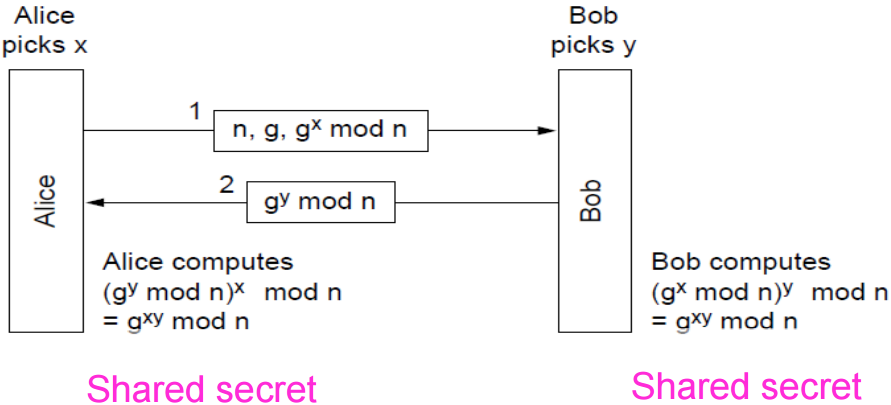
\includegraphics[width=0.90\textwidth]{sharedkey}
            \end{itemize}
          \item Public Key
            \begin{enumerate}
              \item Key Distribution Centre (KDC)
                \begin{itemize}
                  \item Model
                    \newline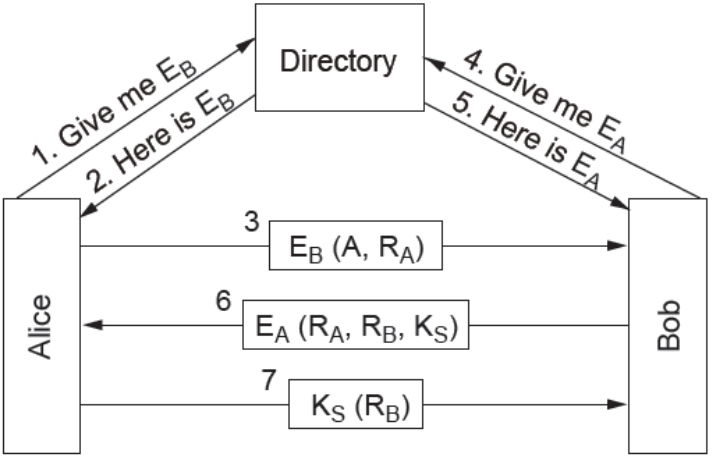
\includegraphics[width=\textwidth]{authpublickey}
                  \item Principle
                    \newline A trusted intermediary is used to facilitate the authentication
                  \item Identity Confirmation
                    \newline Users each share a key with a central key distribution centre, and authenticate to the KDC directly. The KDC then acts as a relay between the two parties.
                  \item Algorithms
                    \begin{itemize}
                      \item Needham Schroeder
                      \item Otway-Rees
                    \end{itemize}
                \end{itemize}
              \item Kerberos
                \begin{itemize}
                  \item Model
                    \newline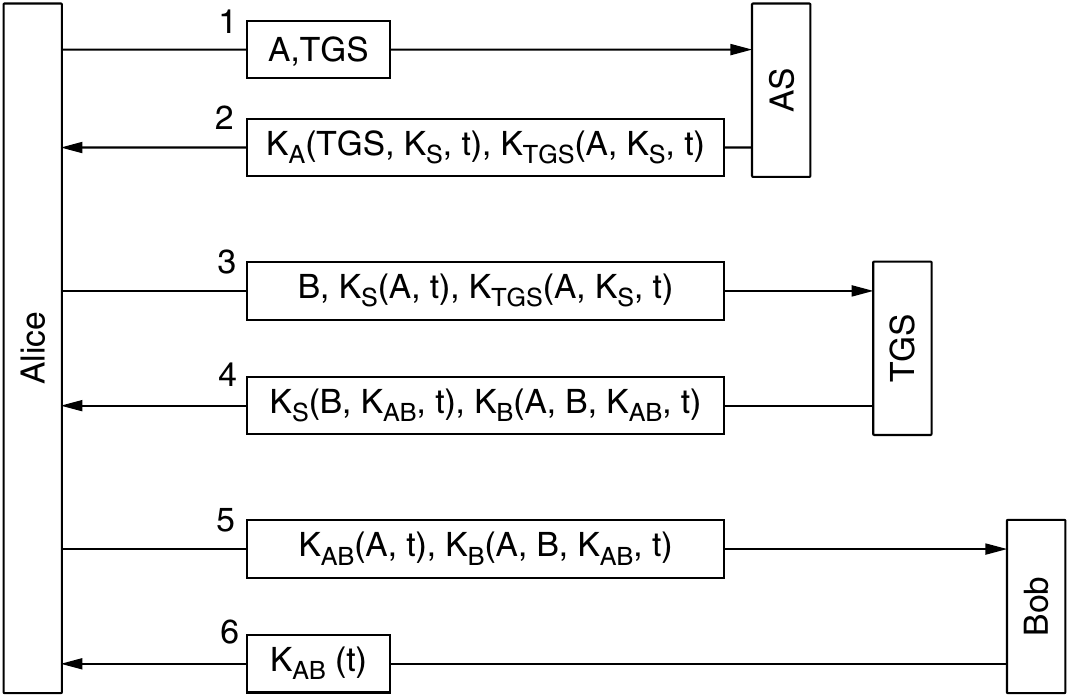
\includegraphics[width=\textwidth]{kerberos}
                  \item Principle
                    \newline A multi-component system is required:
                    \begin{itemize}
                      \item Authentication Server
                      \item Ticket Granting Server
                      \item Recipient
                    \end{itemize}
                  \item Identity Confirmation
                    \newline Authentication is managed centrally, and then party to party communication is facilitated by single use cryptographic tickets.
                    \newline Uses Needham-Schroeder algorithm to minimize insecure connection setup packet exchange
                \end{itemize}
            \end{enumerate}
        \end{enumerate}
        
      \item Firewalls
        \begin{enumerate}
          \item Purpose
            \newline Firewalls, which are positioned at the network boundary, ensures security at the network perimeter by providing a controlled series of route between the internal and external networks
          \item Characteristics
            \begin{itemize}
              \item All \red{inbound and outbound} traffic must transit the firewall
              \item Only \red{authorized traffic} must pass through the firewall
              \item Firewalls should be \red{immune to penetration} themselves.
            \end{itemize}
          \item Reasons for Inspections On Incoming \& Outgoing Packets
            \begin{enumerate}
              \item Incoming
                \newline Anti-virus (likely to be successful for known viruses only)
              \item Outgoing
                \newline Leakage of confidential information (unlikely to be detected if encrypted)
                \newline Denial-of-service attack trace (potentially likely to be detected)
            \end{enumerate}
        \end{enumerate}
        
      \item IPSec
        \begin{enumerate}
          \item Introduction
            \newline IPSec represents one view of how to embed security in the protocol stack - at the network level
          \item Principle
            \newline Encryption is compulsory, but for graceful failover, a null encryption algorithm can be used between points which are not cryptographically inclined
          \item Feature
            \begin{itemize}
              \item Data integrity
              \item Replay attack protection
            \end{itemize}
          \item Algorithm
            \newline IPSec framework allows multiple algorithms and multiple levels of granularity
          \item Connection
            \newline Connection-oriented, with connection being called SA's (security associations)
        \end{enumerate}
        
      \item Virtual Private Network (VPN)
        \begin{enumerate}
          \item Definition
            \newline VPN is a virtual layer on the top of an IP network which provides a secure end-to-end connection over public infrastructure
          \item Common Implementation
            \newline Using a firewall at each end of a connection, setting up a SA to create an IPSec tunnel between the two end points, and then selectively route traffic for the specific destination via the encrypted connection
        \end{enumerate}
        
      \item Wireless Security Context
        \begin{enumerate}
          \item Difficulty
            \newline Difficult to secure because of omnidirectional signal propagation
          \item Wired Equivalency Protocol (WEP)
            \begin{enumerate}
              \item Algorithm
                \newline 40-bit encryption based on RC4
              \item Issues
                \begin{itemize}
                  \item 40 bit encryption is breakable with low-moderate computational resources
                  \item RC4 re-uses keys, so capturing a sufficient volume of encrypted traffic will guarantee key identification 
                \end{itemize}
            \end{enumerate}
          \item Securing Wireless
            \begin{itemize}
             \item MAC Address Filtering
             \item Non-Broadcast SSID
             \item Additional Encryption (128bit WEP)
             \item Multilayered Security
            \end{itemize}
        \end{enumerate}
    \end{enumerate}
    
\end{enumerate}

\end{document}
